\def\difficulty{3}
\sujet{Image Registration}
\index{Registration}

\begin{note}This tutorial aims to implement the Iterative Closest Point (ICP) method for image registration. More specifically, we are going to estimate a rigid transformation (translation + rotation without scaling) between two images.
\end{note}

The different processes will be applied on T1-MR images of the brain in Fig.\ref{fig:registration:enonce:original}.
\begin{figure}[h]
\centering\caption{Original images.}%
\subfloat[brain1]{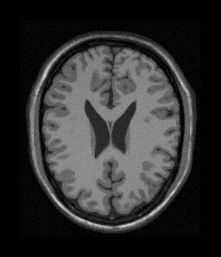
\includegraphics[height=.3\linewidth]{moving}}\hspace{1cm}
\subfloat[brain2]{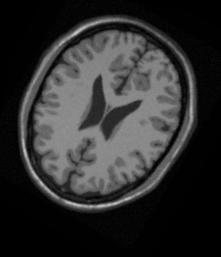
\includegraphics[height=.3\linewidth]{source}}%
\label{fig:registration:enonce:original}%
\end{figure}

\section{Transformation estimation}

A classical method in image registration first consists in identifying and matching some characteristic points by pairs. Thereafter, the transformation is estimated from this list of pairs (displacement vectors).
\subsection{Preliminaries}
Pairs of points are first manually selected.
\begin{qbox}
\begin{itemize}
	\item Read and visualize the two MR images 'brain1' and 'brain2' (moving and source images).
	\item Manually select a list of corresponding points.
\end{itemize}
\end{qbox}

\begin{mcomment}
\begin{mremark}
\minline{cpselect} is a graphical interface dedicated to manual selection of pairs of points. 
\end{mremark}
\end{mcomment}

\begin{pcomment}
\begin{premark}
 There is no built-in function for manual selection of pairs of points. You can use the following points or code your own function, see tutorial \iflabelexists{tutorial:regiongrowing}{\ref{tutorial:regiongrowing}}{about segmentation by region growing.}
 \begin{python}
# define control points
A_points = np.array([[136, 100], [127, 153], [96, 156], [87, 99]]);
B_points = np.array([[144, 99] , [109, 140], [79, 128], [100, 74]]);  
 \end{python}

\end{premark}
\end{pcomment}


\subsection{Rigid transformation}
With this list of pairs ${(p_i,q_i)}_i$, this tutorial proposes to estimate a rigid transformation between these points. It is composed of a rotation and a translation (and not scaling).
For doing that, we make a Least Squares (LS) optimization, which is defined as follows.
The parameters of the rotation $R$ and the translation $t$ minimize the following criterion:
	$$
	C(R,t)=\sum_i ||q_i-R.p_i-t||^2
	$$ 
	\textbf{Calculation of the translation :}\\
	The optimal translation is characterized by a null derivative of the criterion:
	$$
	\frac{\partial C}{\partial t}=-2\sum_i(q_i - R.p_i-t)^{\textsc{T}}=0 \Leftrightarrow \sum_i q_i-R.\left(\sum_i p_i\right) = N.t
	$$
	where $N$ denotes the number of matching pairs.
	By denoting $\bar{p}=\frac{1}{N}\sum_i p_i$ and $\bar{q}=\frac{1}{N}\sum_i q_i$ the barycenters of the point sets
	and by changing the geometrical referential: $p'_i=p_i-\bar{p}$ et $q'_i=q_i-\bar{q}$, the criterion can be written as:
	$$
	C'(R)=\sum_i ||q'_i-R.p'_i||^2
	$$
	The estimated rotation $\hat{R}$ will provide the expected translation:
	\begin{equation}
	\hat{t}=\bar{q}-\hat{R}.\bar{p}\label{eq:registration:enonce:translation}
	\end{equation}
	\textbf{calculation of the rotation by the SVD method:}\\ 
	We will use the following theorem:
	Let $U.D.V^{\textsc{T}}=K$ a singular decomposition of the correlation matrix $K={q'}^{\textsc{T}}.{p'}$, for which the singular values are sorted in the increasing order. The minimum of the criterion: $C(R)=\sum_i ||q'_i-R.p'_i||^2$ is reached by the matrix :
	\begin{equation}\hat{R}=U.S.V^{\textsc{T}} 
	 \label{eq:registration:enonce:rotation}
	\end{equation}
with $S=DIAG(1,\dots,1,\det(U).\det(V))$.


\begin{qbox}
\begin{itemize}\item Code a function that takes as parameters the pairs of points, and returns the rigid transformation elements of rotation $\hat{R}$ and translation $\hat{t}$ as defined in Eqs.\ref{eq:registration:enonce:translation} and \ref{eq:registration:enonce:rotation}. 
	\item Apply the transformation to the moving image.
	\item Visualize the resulting registered image.
	\end{itemize}
\end{qbox}

\begin{mcomment}
\begin{mremark}
\begin{itemize}
 \item See \minline{svd} function.
 \item See \minline{imwarp} and \minline{affine2d} for transformation construction and application.
 \item See \minline{imshowpair} for displaying the registration results.
\end{itemize}
\end{mremark}
\end{mcomment}

\begin{pcomment}
\begin{premark}
 \begin{itemize}\item See \pinline{svd} function from \pinline{scipy.linalg} or \pinline{numpy.linalg}.
  \item See \pinline{cv2.warpAffine} and \pinline{cv2.transform} for transformation application
 \end{itemize}

 
\end{premark}
\end{pcomment}


\section{ICP-based registration}
When the points are not correctly paired, it is first necessary to reorder them before estimating the transformation. In this way, the ICP (iterative Closest Points) consists in an iterative process of three steps: finding the correspondence between points, estimating the transformation and applying it. The process should converge to the well registered image.

\begin{qbox}
To simulate the mixing of the points, randomly shuffle them selected on the first image and perform the registration with the previous method.
\end{qbox}

\begin{mcomment}
\begin{mremark}
See \minline{randperm}. 
\end{mremark}
\end{mcomment}

\begin{pcomment}
\begin{premark}
 See \pinline{np.random.permutation}.
\end{premark}
\end{pcomment}


\begin{qbox}
\begin{enumerate}

	\item From the list of the characteristic points $p$ of the image 'brain1', find the nearest neighbors $q$ in the image 'brain2'. Be careful to the order of the input arguments.
	\item Estimate the transformation $T$ by using the LS minimization coded previously.
	\item Apply this transformation to the points $p$, find again the correspondence between these resulting points $T(p)$ and $q$ and estimate a new transformation. Repeat the process until convergence.
	\item Visualize the resulting registered image.
\end{enumerate}
\end{qbox}

\begin{mcomment}
\begin{mremark}
 Look at \minline{dsearchn} for nearest neighbor search.
\end{mremark}
\end{mcomment}

\begin{pcomment}
\begin{premark}
 Look at \pinline{scipy.spatial.cKDTree} for nearest neighbor search.
\end{premark}
\end{pcomment}


\section{Automatic control points detection}
\index{Features!Detection}
The manual selection of points may be fastidious. Two simple automatic methods for detecting control points are the so-called Harris corners detection or Shi-Tomasi corner detector. 

\begin{mcomment}
\begin{mremark}
The function \minline{detectHarrisFeatures} returns the corners, their coordinates can be retrieved by \minline{corners.selectStrongest(nb_points)}.
\end{mremark}
\end{mcomment}
\begin{pcomment}
\begin{premark}
The function \pinline{goodFeaturesToTrack} returns the corners from the Shi-Tomasi method.
\end{premark}
\end{pcomment}

\begin{qbox}
Replace the manual selection in the two previous parts of this tutorial.
\end{qbox}

Notice that the automatic points detection does not ensure to give the same order in the points of the two images. More generally, other salient points detectors do not give the same number of points, and thus the algorithms have to remove outliers (non matching points). This case is not taken into account in this tutorial.

